\documentclass[12pt,a4paper]{article}
\usepackage[utf8]{inputenc}
\usepackage[spanish]{babel}
\usepackage[T1]{fontenc}
\usepackage{tocbibind} % Bibliografía en el indice
\usepackage{titlesec} % Posibilidad de editar los formatos de chapter
\usepackage{amsmath,amssymb,mathrsfs} % Matemáticas varias
\usepackage{siunitx} % SI de medidas
\usepackage{tabularx} % Para las tablas
\usepackage[title]{appendix} % Para anexos
\usepackage[spanish]{babel} % Para modificar labels por defecto
\renewcommand{\baselinestretch}{1} % Interlineado. 1 es estandar
% --- Arreglos varios para la inclusion de imagenes
\usepackage{float}
\usepackage[pdftex]{graphicx}
\usepackage{subfigure}
\usepackage{graphicx}
\graphicspath{{T:/Tom/Facultad/Logos/}{T:/Tom/Facultad/Materias/EDII/TPs/LED/Imagenes/}}
\usepackage[usenames,dvipsnames]{color}
\DeclareGraphicsExtensions{.png,.jpg,.pdf,.mps,.gif,.bmp}
% --- Para las dimensiones de los márgenes etc
\frenchspacing \addtolength{\hoffset}{-1.5cm}
\addtolength{\textwidth}{3cm} \addtolength{\voffset}{-2.5cm}
\addtolength{\textheight}{4cm}
% --- Para el encabezado
\setlength{\headheight}{33pt}
\usepackage{fancyhdr}
\fancyhead[R]{\includegraphics[height=1cm]{logo_fcefyn_nuevo.jpg}}\fancyhead[L]{\includegraphics[height=1cm]{unc1_a.jpg}}\fancyhead[C]{Electrónica Digital II} \fancyfoot[C]{Página \thepage} \renewcommand{\footrulewidth}{0.4pt}
\pagestyle{fancy}
% --- Para las tablas
\usepackage{multirow} % Juntar filas
\newcolumntype{L}[1]{>{\raggedright\arraybackslash}p{#1}} % Justificar Izq
\newcolumntype{C}[1]{>{\centering\arraybackslash}p{#1}} % Justificar Centrar
\newcolumntype{R}[1]{>{\raggedleft\arraybackslash}p{#1}} % Justificar Der
\usepackage[numbered]{bookmark} % Para que figure las secciones en el PDF
\usepackage{listings} % Para poner código 
\usepackage{enumitem} % Para editar las propiedades de los items
\usepackage{color}
\usepackage[bottom]{footmisc} % Para las notas al pie de la página
\lstset{frame=single} % Código en un cuadro
% --- Para Anexo
\addto\captionsspanish{%
  \renewcommand\appendixname{ANEXO}
  \renewcommand\appendixpagename{ANEXOS}
}
% -------------------------------------------------------- %
% Definicion de colores para el codigo
\lstdefinelanguage{XML}
{
  basicstyle=\ttfamily\footnotesize,
  morestring=[b]",
  moredelim=[s][\bfseries\color{Maroon}]{<}{\ },
  moredelim=[s][\bfseries\color{Maroon}]{</}{>},
  moredelim=[l][\bfseries\color{Maroon}]{/>},
  moredelim=[l][\bfseries\color{Maroon}]{>},
  morecomment=[s]{<?}{?>},
  morecomment=[s]{<!--}{-->},
  commentstyle=\color{DarkOliveGreen},
  stringstyle=\color{blue},
  identifierstyle=\color{red}
}

\renewcommand{\lstlistingname}{Código}

% -------------------------------------------------------- %

\begin{document}

\begin{titlepage}
    \begin{center}
        \vspace*{1cm}
        
        \Large
        \textbf{Universidad Nacional de Córdoba\\
        		Facultad de Ciencias Exatas, Físicas y Naturales}
        
        \vspace{0.5cm}
        \includegraphics[width=0.5\textwidth]{logo_caratula.png}
        
        \vspace{1.5cm}
        
        \textbf{Primer Trabajo Práctico}\\
        Electrónica Digital II\\
        Docente: Ing. Martín Del Barco
        
        \vfill  
        
        \vspace{0.8cm}
        

        
        \Large
        Losano Quintana, Juan Cruz\\
        Piñero, Tomás Santiago\\
        Ingeniería en Computación\\
        Año 2019\\
        
        
    \end{center}
\end{titlepage}
% -------------------------------------------------------- %

% --- Tabla de contenidos
\tableofcontents
\setcounter{secnumdepth}{1}

% -------------------------------------------------------- %

\newpage
\renewcommand{\baselinestretch}{1}
\setlength{\parskip}{0.5em}

\section{Enunciado}
	Realizar un programa que permita sumar dos valores de cuatro bits cada uno, ingresados desde puertos configurados como entradas. El resultado debe mostrarse mediante cuatro LEDs conectados a puertos configurados como salidas. En caso de producirse un acarreo del tipo "\emph{Digit Carry}", un quinto LED empezará a parpadear indefinidamente con un periodo de aproximadamente un segundo prendido y un segundo apagado. A partir de ese instante ya no podrán realizarse más sumas, salvo que se realice un reset del microcontrolador.
	
	Armar en la protoboard el circuito totalmente funcional para ser presentado y evaluado en clase.
	
	Adjuntar una foto de la hoja que muestre el diagrama de todas las conexiones realizadas en el diseño con el cálculo del valor de las resistencias limitadoras de los puertos de salida y el cálculo del tiempo de parpadeo de los bucles anidados utilizados para la frecuencia de reloj elegida.

\newpage

\section{Desarrollo}
\subsection{Introducción}
	Para la realización del trabajo práctico se utilizaron los siguientes materiales:
	
	\begin{itemize}[leftmargin=1.5cm,nosep]
	\item PIC16F887.
	\item Cristal de \SI{4}{\MHz}.
	\item LEDs de color verde, amarillo y rojo.
	\item Resistencias de \SI{1}{\kilo\ohm} y \SI{330}{\ohm}.
	\item Dos capacitores de \SI{2}{\pF}.
	\item Dos Deep Switch de cuatro llaves.
	\item Un pulsador.
	\end{itemize}

	Al ser dos números de cuatro bits, el resultado será de cinco bits en el peor de los casos, por lo tanto se pueden utlizar dos puertos del PIC para implementar el circuito, ya  que éste posee cuatro puertos de ocho bits.
	
	Se seleccionó el puerto B como puerto de entrada de ambos números y el puerto A como salida para mostrar el resutlado de su suma.
	
\subsection{Cálculos de resistencias}
	Antes de realizar la implementación del circuito se deben calcular las resistencias tanto para las entradas como para las salidas del PIC.
	
\subsubsection{Pull-ups}
	La limitación de la corriente en el puerto de entrada se llevó a cabo por medio de \emph{pull-ups}.
	
\subsubsection{LEDs}
	Las resistencias para los LEDs se llevaron a cabo de la siguiente manera:
	
\section{Implementación}
\subsection{Diagramas de flujo}
	\subsubsection{Programa principal}
	\subsubsection{Delay}
	\subsubsection{Parpadeo}
	
\newpage
\subsection{Esquema del circuito}

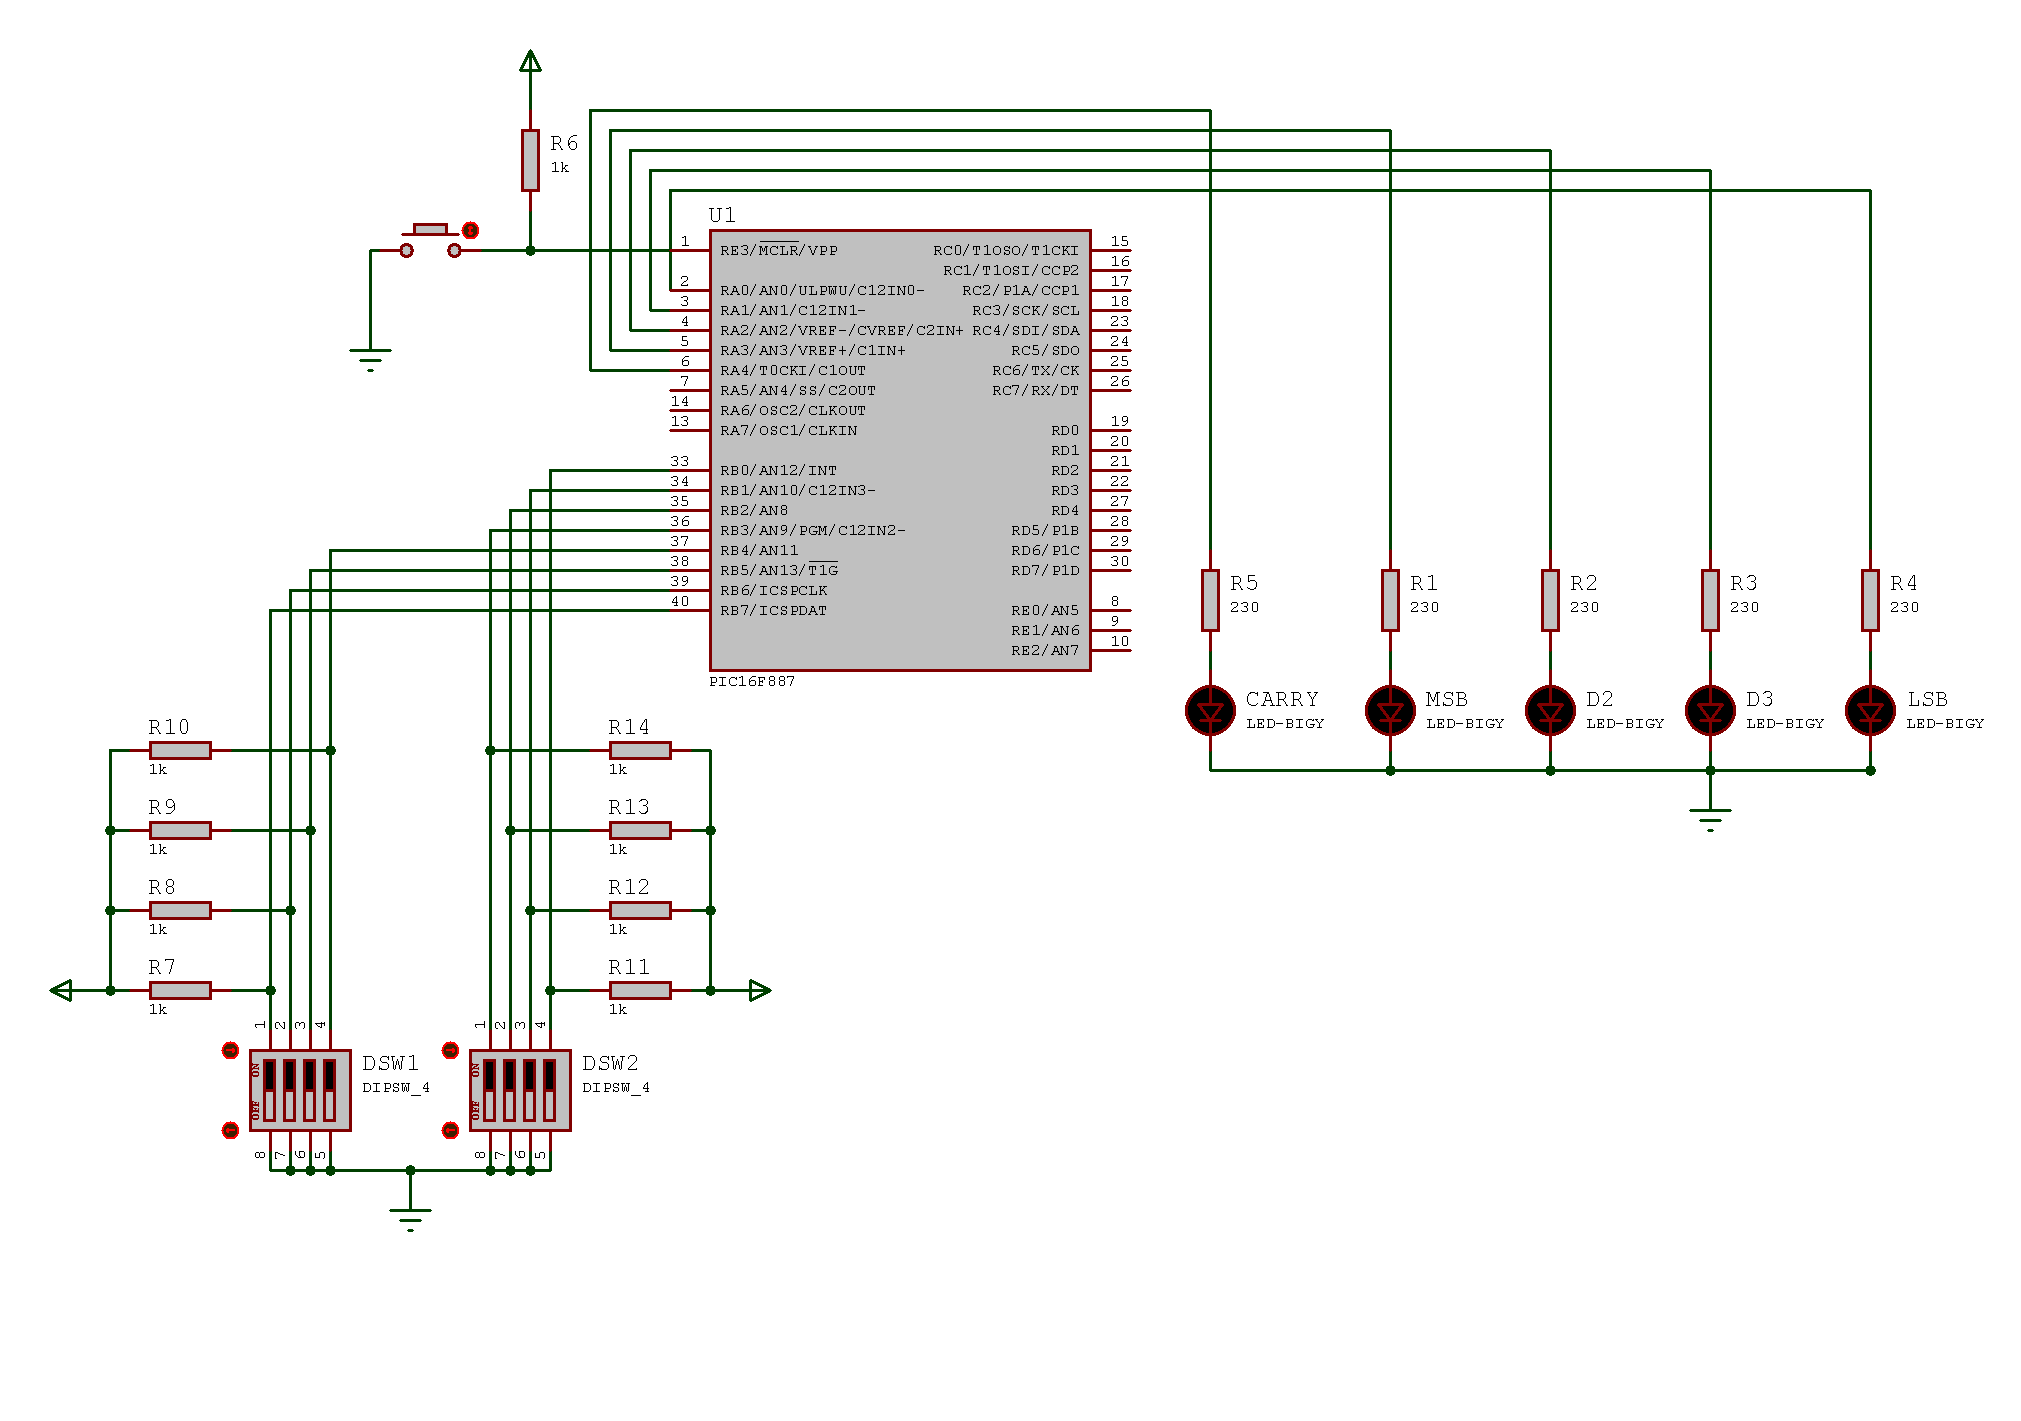
\includegraphics[angle=90,origin=c,scale=0.33]{circuito.png}

	
\end{document}